
La concretizzazione della soluzione al problema esposto è l’applicativo \textbf{PineSU}~\cite{pinesu-github-21}. \\
PineSU si presenta come un software \emph{lightweight} scritto in Javascript e che sfrutta il runtime Node.js.
L’applicazione va a considerare gli insiemi di file come delle entità chiamate \\
\textbf{Storage Unit} (SU) con cui va ad inglobare logicamente una repository Git, cotruendo,
tramite la definizione di alcuni metadati, una struttura introno ad essa. \\
Queste SU sono le unità su cui si andranno ad effettuare le singole
operazioni, eccetto la registrazione su blockchain che si svolgerà collettivamente con l’ausilio di accumulatori crittografici. 

Vedremo come il ciclo di vita di una SU sia scandito dai \textbf{Blockchain Synchronization Point} (BSP),
ovvero gli eventi che si generano quando si decide di andare a registrare lo stato e la presenza di una SU nella blockchain, inserendola
all’interno gruppi di suoi simili chiamati \textbf{Storage Group} (SG). Questi finiranno poi nella grande struttura chiamata \textbf{Merkle Calendar} (MC).
Infine, la root di questo MC sarà salvata nella blockchain (nell’implementazione attuale, quella Ethereum), da qui in poi sarà possibile, in qualsiasi momento, ricostruire un MC in quel preciso istante in cui un nuovo BSP è stato creato e verificare se la root di questa ricostruzione è presente nel registro.

\section{Workflow}
\label{sec:work}

PineSU segue una filosofia di workflow che ricalca quella di Git,
infatti tramite l’applicativo si può operare su singole Storage Unit, ognuna con uno stato potenzialmente
diverso dall’altra. Ciò fa si che il workflow sia molto legato al ciclo di vita di una singola SU, la quale
a seconda del suo stato permetterà di fare alcune operazioni anziché altre.

\begin{figure}[H]
    \centering
    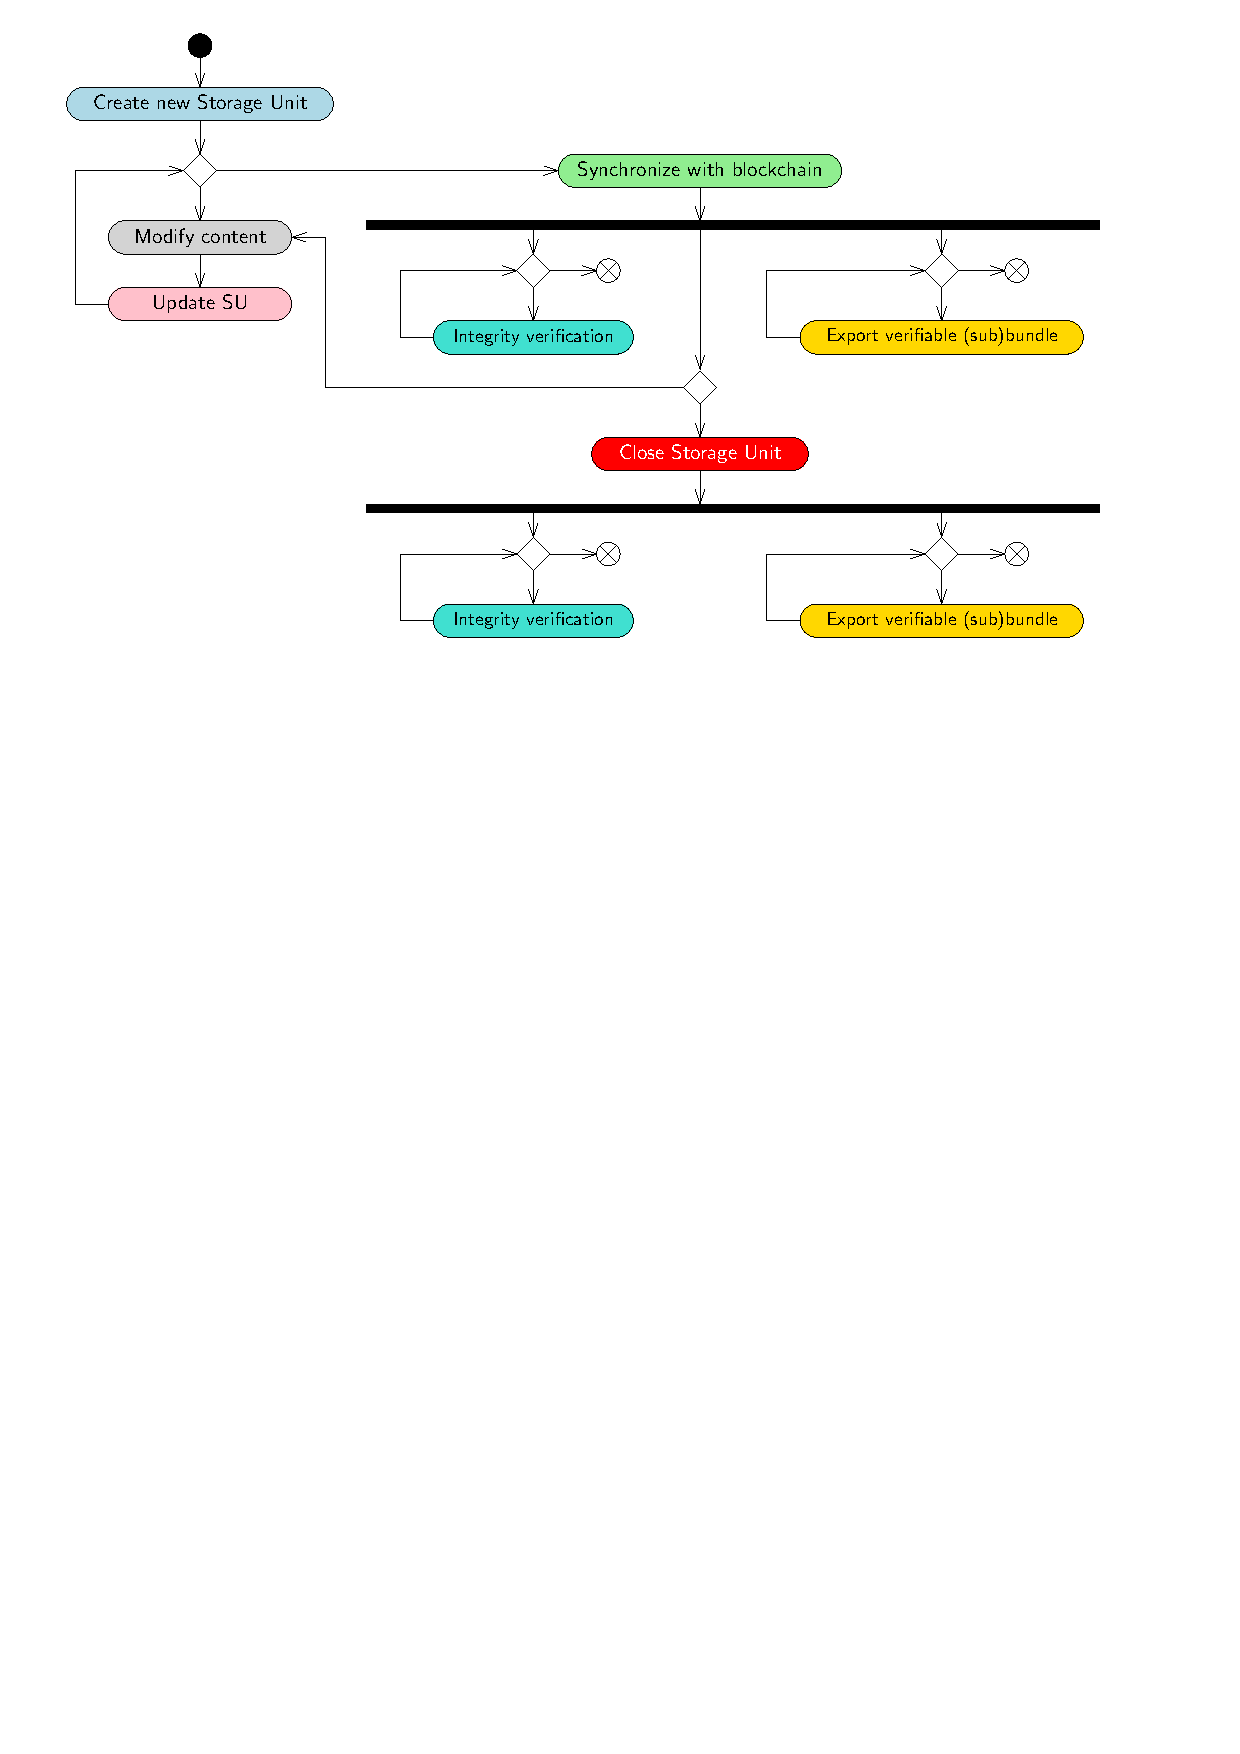
\includegraphics[width=0.98\textwidth]{Figures/activityDiag}
    \caption{\small{
    Workflow dell’applicativo sotto forma di Activity Diagram.
    } % end small
    } % end caption
    \label{fi:workflow}
\end{figure}

Possiamo vederne una rappresentazione in Fig.~\ref{fi:workflow}, si parte da una directory del nostro file
system e, tramite PineSU, la si trasforma in una Storage Unit (\emph{Create new Storage Unit}) calcolandone
anche i metadati in modo da rendere già possibili registrazioni e verifiche.
Dopo questa operazione potrebbero accadere i due eventi che seguono: 
\begin{enumerate}
    \item Il contenuto della Storage Unit potrebbe venire modificato,
    a questo punto è necessario, se si vogliono registrare anche i nuovi cambiamenti,
    andare ad effettuare un ricalcolo (\emph{Update SU}), dopo di ciò
    si torna alla possibilità dei tre eventi;
    \item Potremmo scegliere di sincronizzare la SU nella blockchain (\emph{Synchronize with blockchain}),
    questo avviene in realtà tramite due fasi che vedremo in seguito, tuttavia
    questa scelta ci permette in seguito di eseguire qualsiasi operazione lo stesso,
    eccetto il ricalcolo nell’eventualità che questa SU sia stata chiusa precedentemente.
\end{enumerate}

Una volta che una SU è stata registrata nella blockchain o chiusa si aprono altre
due possibili azioni da poter compiere: la verifica d’integrità (\emph{Verify integrity with blockchain}),
sia offline che online, e l’esportazione di sottoinsiemi di file dalla SU (\emph{Export blockchain verifiable bundle}),
munendoli con i dati necessari per permettere verifiche d’integrità da parte di terzi
anche senza disporre dell’intera SU.

Una terza operazione da effettuare una sola volta in seguito a una registrazione è la chiusura
(\emph{Close Storage Unit}).
Una SU è aperta (\textbf{Open}) se modificabile e ricalcolabile liberamente,
chiusa (\textbf{Closed}) se la modifica, il ricalcolo e un’eventuale chiusura
successiva non possono essere eseguiti. Dopo la chiusura, a cui dovrebbe
seguire una regsitrazione su blockchain, potranno essere eseguite
in pratica le stesse operazioni eccetto, ovviamente, quella del ricalcolo;

Possiamo osservare il workflow appena descritto anche in Fig.~\ref{fi:stateDiag}, dove il diagramma degli
stati di una singola Storage Unit riflette le operazioni appena descritte.
Appena creata possiamo infatti riferirci ad essa come una Storage Unit \textbf{Updated Unsynchronized Open},
ovvero aperta e non sincronizzata alla blockchain, tuttavia aggiornata in quanto gli hash sono stati calcolati
sulla situazione corrente dei file contenuti. Sincronizzandola diventa una SU \textbf{Updated Synchronized Open},
su cui possiamo eseguire operazioni di verifica ed esportazioni senza cambiare però il suo stato.
Modificando un file esternamente, in entrambi gli stati che abbiamo visto, si entra in uno stato da cui si
può uscire solamente eseguendo un ricalcolo: ovvero quello di SU \textbf{Not-updated Unsynchronized Open}.
Una chiusura unita con una registrazione su blockchain fanno diventare la SU
\textbf{Updated Synchronized Closed}, uno stato in cui la modifica non è permessa.


\begin{figure}[H]
    \centering
    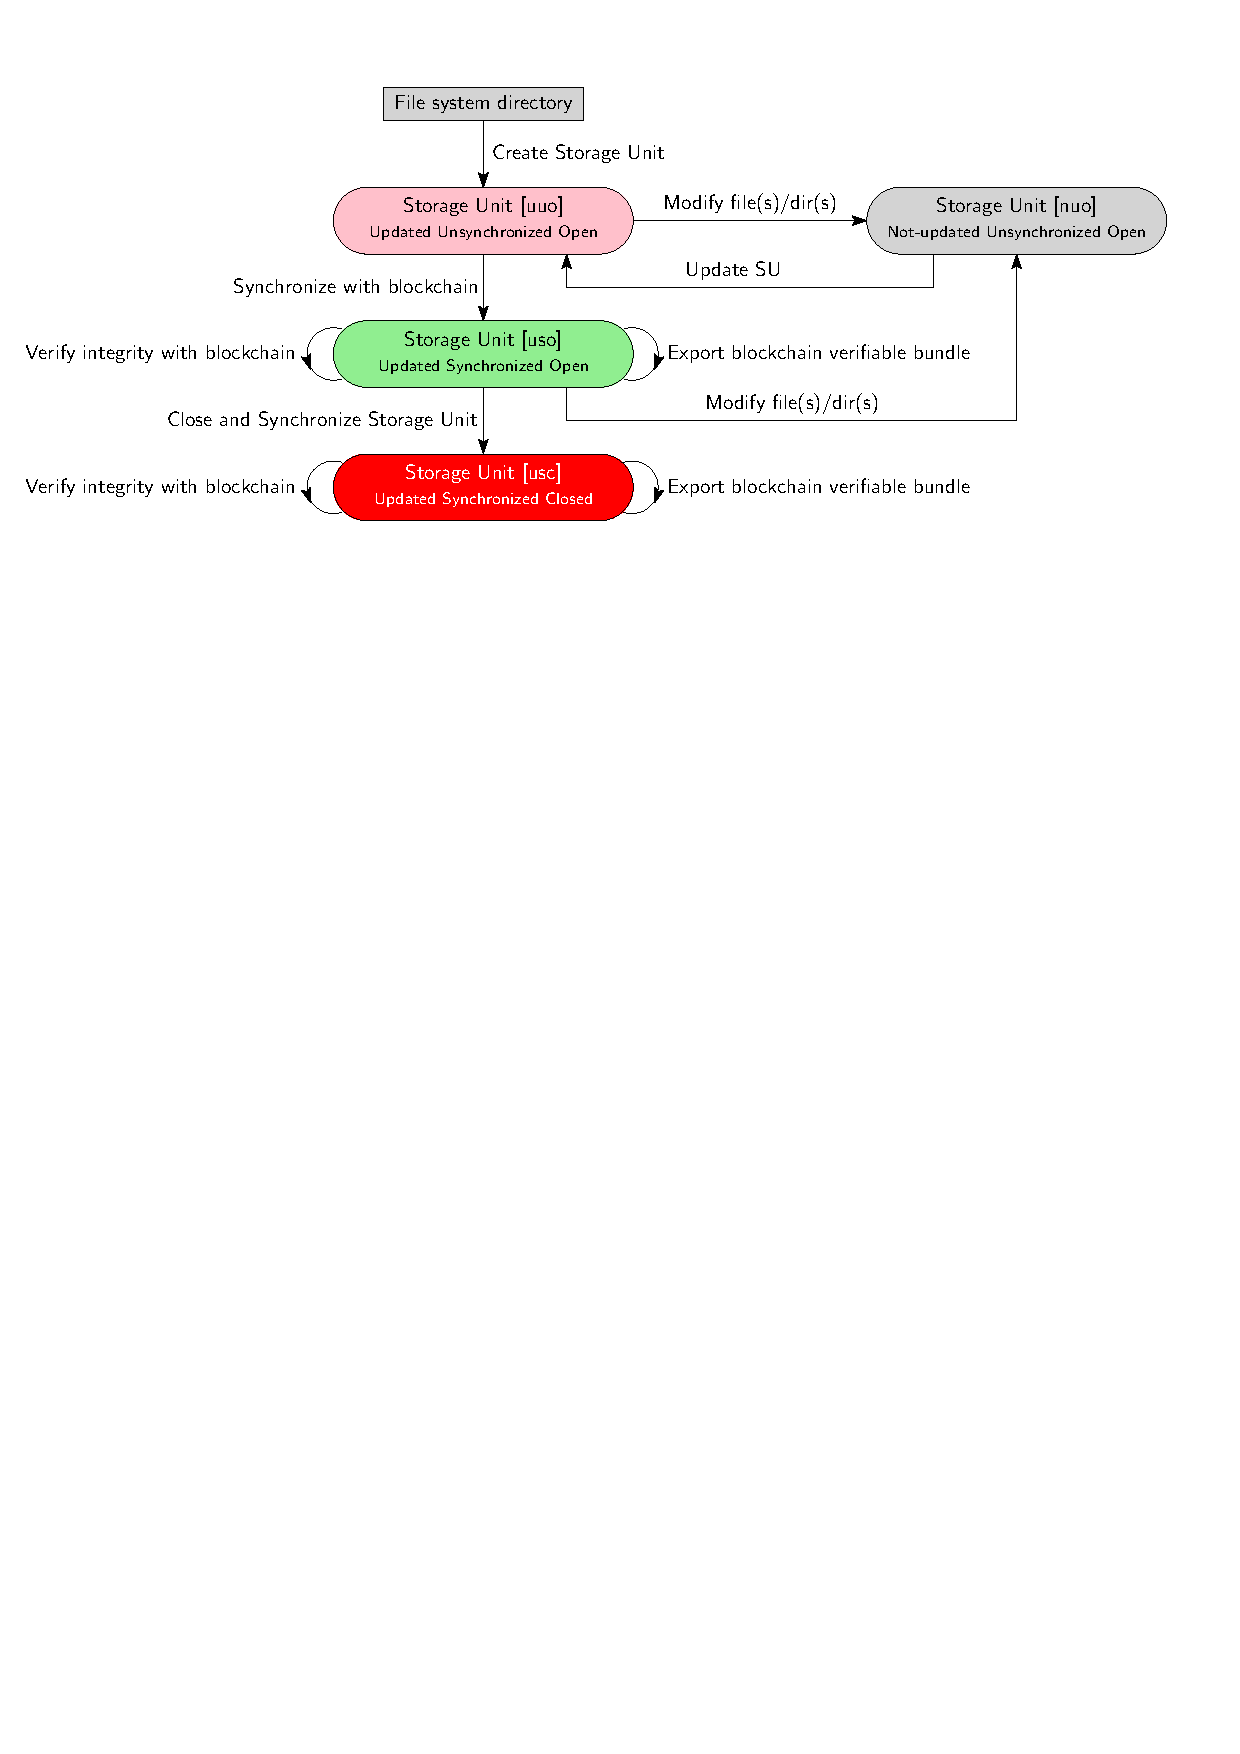
\includegraphics[width=0.98\textwidth]{Figures/stateDiag2}
    \caption{\small{
    Ciclo di vita di una Storage Unit sotto forma di State Diagram.
    } % end small
    } % end caption
    \label{fi:stateDiag}
\end{figure}

\section {Architettura}
\indent
Il sistema va ad interfacciarsi con il client Git e con l’API \textsf{web3.js} per la comunicazione
con la blockchain Ethereum, possiamo descrivere la sua architettura come in Fig.~\ref{fi:arch}, dove troviamo i componenti principali:
\begin{itemize}
    \item \emph{PineSU \textbf{CLI} (Command Line Interface)}. L’interazione con PineSU da parte degli utenti avviene attraverso un emulatore di terminale, analogamente a come avviene con Git, di una macchina avente Node.js installato\footnote{L’interfaccia si basa sul modulo npm Inquirer.js ~\cite{inquirer-github-21}}, tuttavia con un’interazione più guidata rispetto al noto VCS. Oltre al permettere l’uso delle normali funzioni di PineSU, questo modulo permette anche l’inserimento di un qualsiasi comando di Git, in modo da rendere l’utilizzo diretto di quest’ultimo non necessario durante una tipica sessione di lavoro.
    \item \emph{PineSU \textbf{BEL} (Back End Logic)}. Questo componente è il nucleo di PineSU\footnote{Il componente si basa su alcuni moduli npm per opertazioni di supporto ~\cite{adm-zip-github-21}~\cite{chalk-github-21}~\cite{merkle-tools-github-21}}. Gestisce tutte le SU e controlla la comunicazione con la blockchain e il client Git locale.
    Il client Git viene utilizzato inoltre per interagire indirettamente con i server Git remoti.
    Il modulo BEL, in aggiunta, si occupa della gestione dei due Storge Group, Open (OSG) e Closed (CSG), e
    mantiene il Merkle Tree dinamico chiamato Merkle Calendar che permette di recuperare efficientemente
    l’hash registrato in blockchain per un qualsiasi BSP. La gestione del salvataggio remoto del Merkle Calendar avviene tramite una repository Git scelta dall’utente.
    \item \emph{PineSU \textbf{EC} (Ethereum Connector)} Si interfaccia con il modulo \textsf{web3.js}~\cite{web3js-github-21}~\cite{web3js-doc-21}. 
    \item \emph{PineSU \textbf{GC} (Git Connector)} Si interfaccia con il modulo \textsf{simple-git}~\cite{simple-git-github-21}. 
    \item \emph{PineSU \textbf{SM} (Smart Contract)} Questo modulo entra in gioco solamente nel caso di una registrazione “forte” di una Storage Unit nella blockchain, in una fruizione standard dell’applicativo non entrerà probabilmente in azione.
\end{itemize}

\begin{figure}[H]
    \centering
    \includegraphics[width=0.98\textwidth]{Figures/PineSU-architecture}
    \caption{\small{
    Rappresentazione dell’architettura ad alto livello di PineSU. 
    Le frecce nere sono messaggi scatenati dalle entità sorgente corrispondenti
    mentre le frecce grigie sono risposte passive dell’entità interrogata.
    } % end small
    } % end caption
    \label{fi:arch}
\end{figure}

\section{Moduli in dettaglio}
\subsection{PineSU CLI}

Il modulo si occupa di creare l’effettiva interfaccia utente con cui è possibile interagire,
le domande vengono create dal modulo apposito “inquirer”, dove sono definite
insieme alle risposte possibili e ai controlli di consistenza delle risposte date dall’utente.

Dopo un setup una tantum in cui all’utente vengono chieste informazioni come gli indirizzi dei
suoi due wallet, a seconda delle scelte dall’utente, la prima di cui sarà quella dell’effettiva
operazione da eseguire (Fig.~\ref{fi:menu}), il modulo va a delineare il workflow preciso che descrive il ciclo vitale
di una SU, il tutto richiamando all’occorrenza le librerie del modulo \emph{PineSU BEL}. 

\begin{figure}[H]
    \centering
    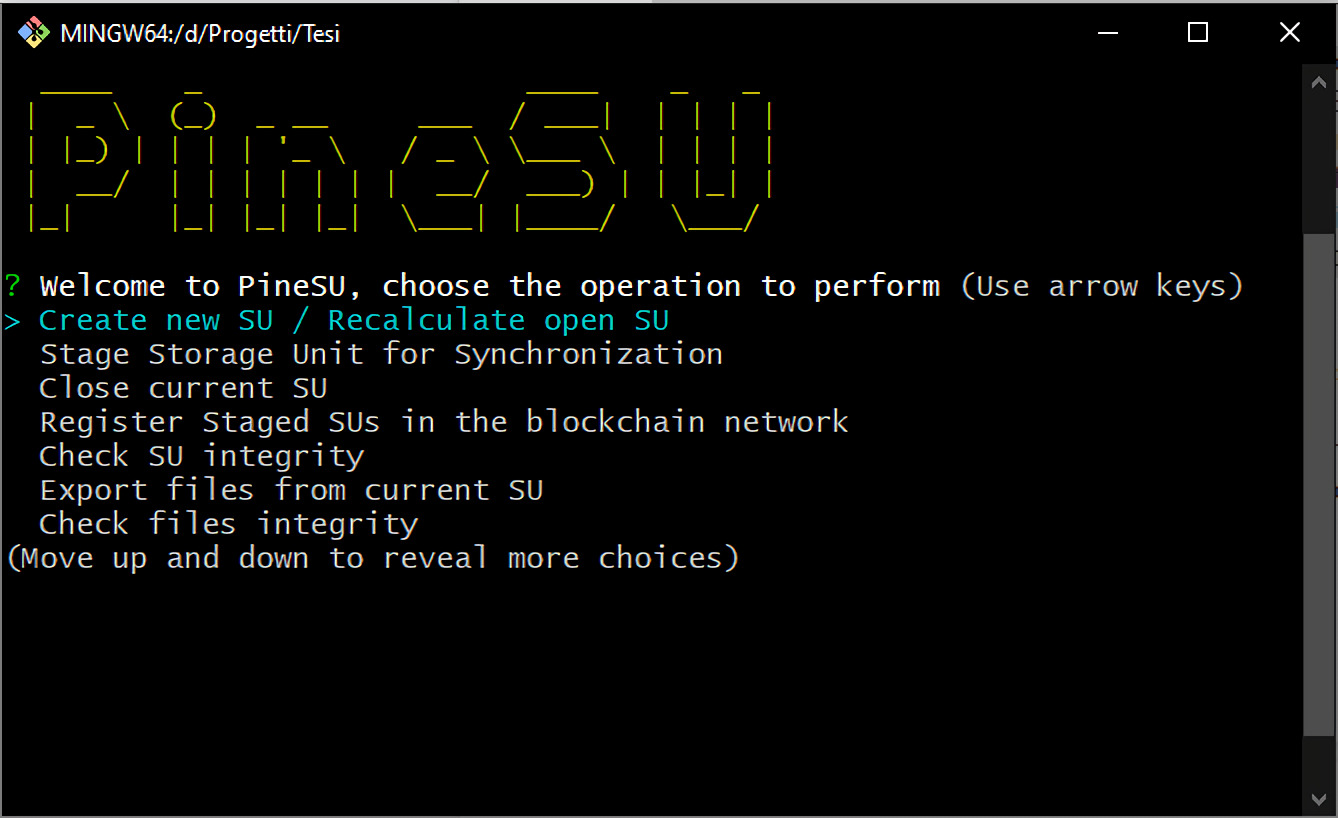
\includegraphics[width=0.98\textwidth]{Figures/menu}
    \caption{\small{
    Menù principale dell’applicativo con la scelta dell’operazione da effettuare.
    } % end small
    } % end caption
    \label{fi:menu}
\end{figure}

\newpage

\subsection{PineSU BEL}

Questo modulo è il nucleo centrale del software, si occupa dell’effettiva comunicazione con i connettori per Git e per la blockchain, del gestire il File System andando a leggere e scrivere i file all’interno delle Storage Unit, di assegnare stringhe crittografiche ai singoli file e di creare e gestire le strutture di accumulazione crittografica.

Per la prima delle operazioni sopra citate troviamo due librerie, rispettivamente \textbf{GitLogic} e \textbf{EthLogic}, le quali si occupano essenzialmente di creare oggetti delle rispettive classi di connettori, reperire tramite altre librerie le informazioni necessarie, chiamare le funzioni dei connettori con gli input dovuti e gestire gli output in maniera coerente con ciò che necessita \emph{PineSU CLI}.

Andiamo ora a vedere le due classi che si occupano di creare e gestire le strutture di memorizzazione che il programma utilizza: \textbf{Files} e \textbf{TreeList}.
Files si occupa della lettura e scrittura di file JSON e della lettura dei file di cui andrà calcolata la stringa di hash corrispondente. Questi file JSON corrispondono ai descrittori delle SU (riguardanti la creazione e la registrazione su blockchain), alle informazioni sull’utente utilizzatore e alle strutture degli accumulatori crittografici.
TreeList si occupa del reperimento delle stringhe di hash e del calcolo dei Merkle Tree binari.
Essi sono fondamentali per varie operazioni che vanno dal calcolo degli hash delle directory alla creazione dei tre accumulatori crittografici che andremo ora a descrivere.

Il primo è il semplice SU Merkle Tree, necessario per il calcolo dell’hash corrispondente alla Storage Unit, che altro non è che un Merkle Tree binario in cui ogni foglia corrisponde a un file o una directory contenuta nella SU. Questo MT verrà utilizzato anche nella fase di esportazione per generare le proof dei file esportati che serviranno per un eventuale controllo d’integrità singolo.

Il secondo è lo Storage Group, di cui ne esistono due, un \textbf{Open} (OSG) e un \textbf{Closed} (CSG). Si tratta essenzialmente di due MT binari in cui ogni foglia corrisponde all’hash di una Storage Unit \textbf{Staged} (ovvero preparata per la registrazione collettiva, ne parlremo meglio nella \autoref{sub:stage}), la differenza tra i due alberi è nel loro contenuto, uno contiene le SU Open, l’altro le SU Closed, differenza già discussa nella \autoref{sec:work}. Le root di questi alberi verranno poi salvate all’interno della prossima struttura come foglie.

Il terzo e più importante è il \textbf{Merkle Calendar}, formato da due sottoalberi in cui vengono accolte come foglie rispettivamente le root delle istanze di OSG e di CSG. Le radici di questi due sottoalberi hanno come figli dei nodi corrispondenti agli anni, i quali a loro volta hanno come figli dei nodi corrispondenti ai mesi, i figli dei mesi saranno infine le foglie corrispondenti a ciò che chiamiamo \textbf{Blockchain Synchronization Point} (BSP) in quanto nodi contenenti un timestamp e la root dello SG corrispondente.

Per ogni BSP, sappiamo che c'è stata la registrazione su blockchain della blockchain
della root dell'MC in quel momento.
Possiamo vedere, anche grazie a Fig.~\ref{fi:umlMC}, come questa struttura sia implementata tramite tre classi:

\begin{itemize}
    \item \textbf{MerkleCalendar}: contiene i riferimenti alle due radici dei sottoalberi e mette a disposizione varie funzioni per la ricerca di hash e reperimento di determinati valori della root in un certo BSP.
    \item \textbf{InternalCalendar}: corrisponde a un nodo interno dell’albero, quando si aggiungono figli si può scegliere di effettuare il ricalcolo del loro hash in modo da non doverlo calcolare successivamente (semplifica l’operazione di reperimento dell’hash di un certo BSP).
    \item \textbf{LeafCalendar}: corrisponde a una foglia dell’albero.
\end{itemize}


\begin{figure}[H]
    \centering
    \resizebox{0.9\textwidth}{!}{
        \begin{tikzpicture}
            \begin{class}[text width=14cm]{MerkleCalendar}{0,0}
                \attribute{}
                \operation{+ addRegistration(name: string, hash: string, date: Date, closed: boolean): void}
                \operation{+ getBSPRoot(hash: string, oHash: string, cHash: string): string}
                \operation{+ getTrees(): [Array, Array]}
            \end{class}
            \begin{class}[text width=9.5cm]{InternalCalendar}{4,-4.5}
                \attribute{- name : string}
                \attribute{- category : int}
                \attribute{- parent : InternalCalendar}
                \attribute{- category : int}
                \attribute{- hash : string}
                \operation{constructor(name: string, category: int, parent: Object)}
                \operation{+ addChild(node: Object) : void}
                \operation{+ calculateHash() : void}
                \operation{+ getChildByName(name: string) : Object}
                \operation{+ findNode(hash: string) : Object}
            \end{class}
            \begin{class}[text width=15cm]{LeafCalendar}{2,-12.5}
                \attribute{- name : string}
                \attribute{- day : int}
                \attribute{- hour : InternalCalendar}
                \attribute{- minute : int}
                \attribute{- hash : string}
                \operation{constructor(name: string, day: int, hour: int, minute: int, hash: string, parent: Object)}
            \end{class}
            \composition{MerkleCalendar}{open, closed}{2}{InternalCalendar};
            %\aggregation{InternalCalendar}{children}{0..*}{LeafCalendar};
            %\aggregation{LeafCalendar}{parent}{0..1}{InternalCalendar};
            \aggregation{[xshift=2cm] InternalCalendar.south}{0..*}{children}{[xshift=2cm] LeafCalendar.north};
            \composition{[xshift=-2cm] LeafCalendar.north}{1}{parent}{[xshift=-2cm] InternalCalendar.south};
            %\aggregation{[xshift=-2cm] A}{second}{1}{[xshift=-2cm] B.north};
            \selfAssociation{InternalCalendar}{parent}{0,1};
        \end{tikzpicture}
    }
    \caption{Rappresentazione UML delle classi descritte} \label{fi:umlMC}
\end{figure}

\newpage

\subsection{Excursus sul Merkle Calendar}

In Fig.~\ref{fi:mcIPE} possiamo osservare un possibile Markle Calendar.
Nell’esempio è stato esplorato il mese di Febbraio 2021 e lì troviamo tre BSP:
esse corrispondono a tre registrazioni della root dell’intero MC su blockchain, ovviamente
sempre diversa dato che l’hash root si calcola con gli hash delle sue foglie.

\begin{figure}[H]
    \centering
    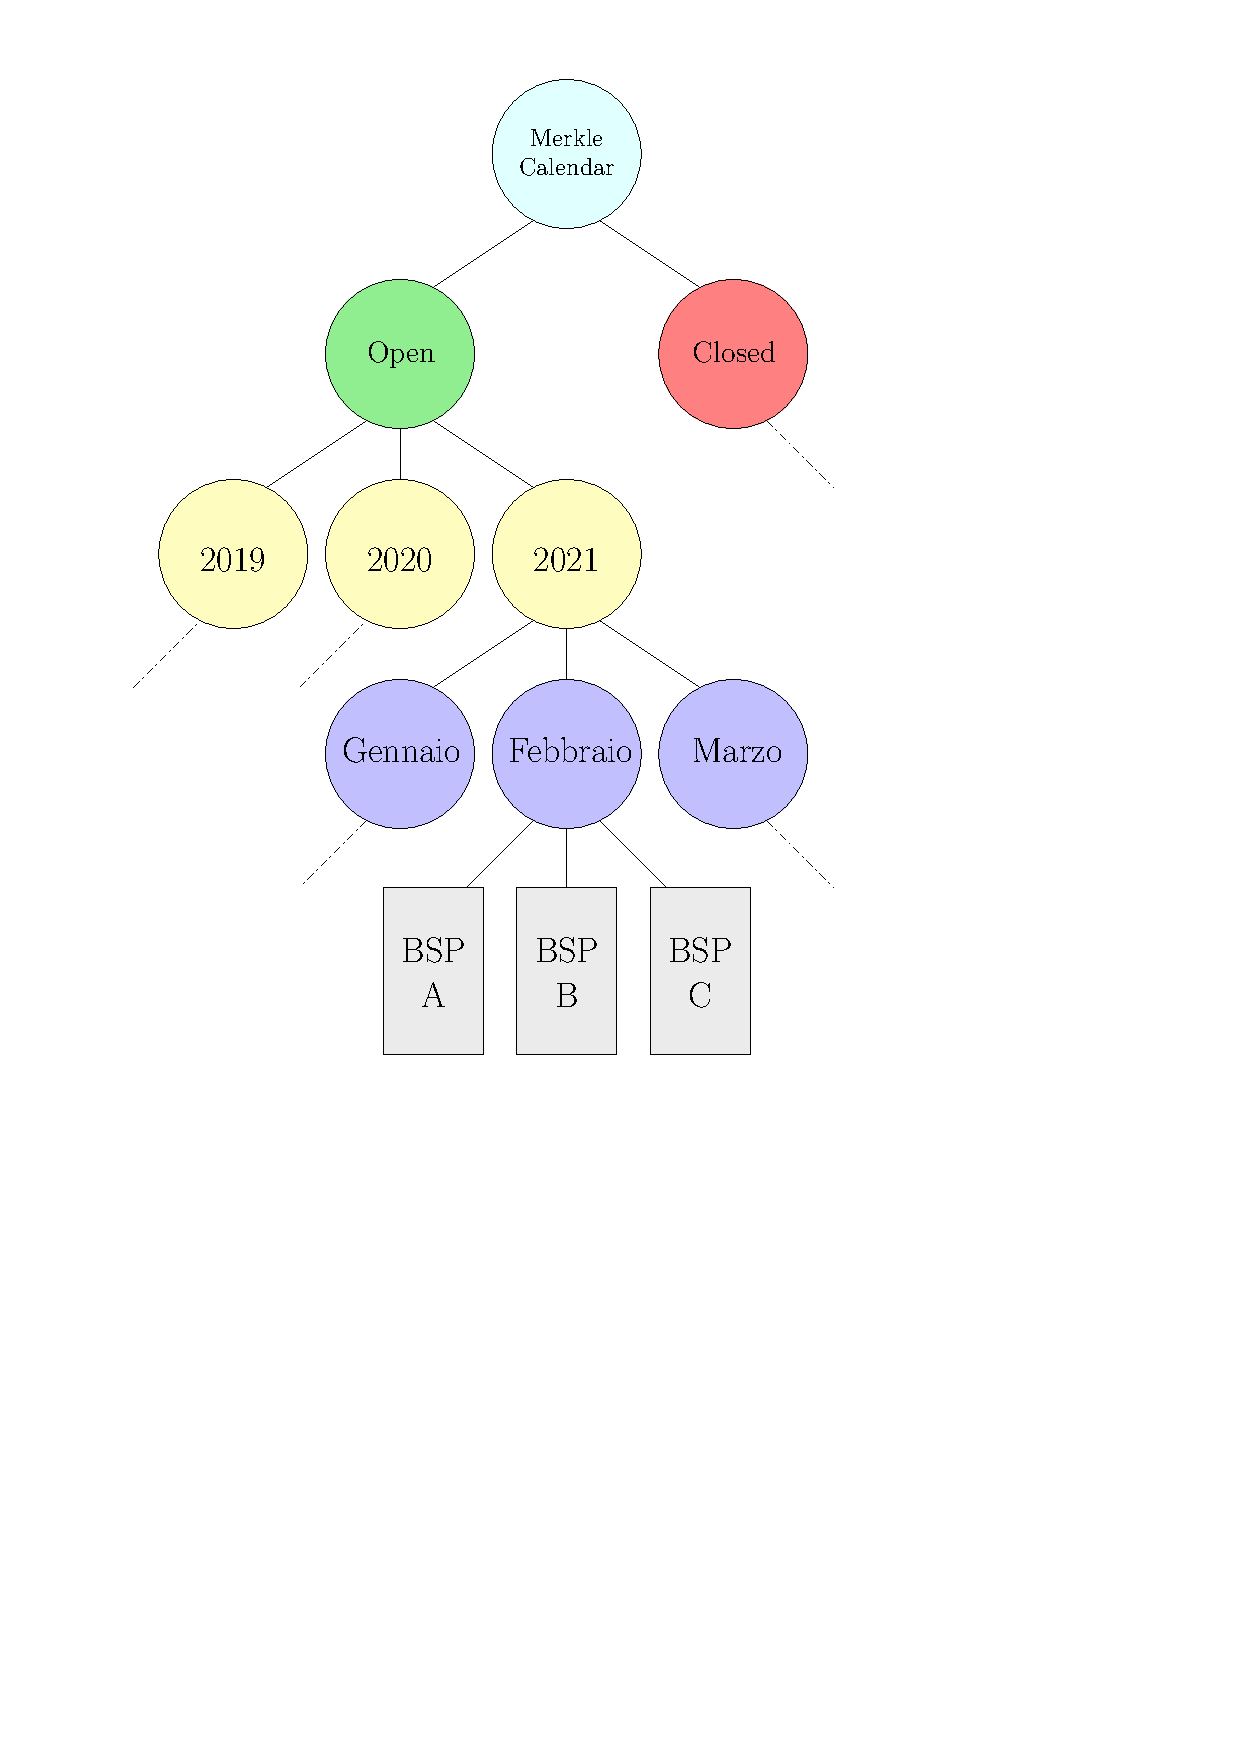
\includegraphics[width=0.5\textwidth]{Figures/mc1}
    \caption{\small{
    Rappresentazione grafica di un Merkle Calendar.
    } % end small
    } % end caption
    \label{fi:mcIPE}
\end{figure}

Ogni volta che un nuovo BSP viene inserito per la prima volta si avvia la procedura di
ricalcolo dell’hash di ognuno dei suoi antenati in modo da non dover effettuare il calcolo
dell’hash di gran parte dell’albero nella fase di reperimento.

Nel momento in cui ognuna di queste tre BSP è stata inserita nell’albero essa era la foglia più
giovane, ergo se volessimo calcolare la root del MC in una data BSP ci basterebbe non
considerare tutto ciò che è stato inserito successivamente, andando ad escludere una
partizione di estrema destra dal sottoalbero radicato in Open (in questo caso).

\newpage

Ipotizziamo di voler recuperare la MC root nel momento in cui è stata inserita BSP B:
\begin{enumerate}
    \item Calcoliamo l’hash di Febbraio tramite l’hash di BSP a e di BSP B;
    \item Calcoliamo l’hash del 2021 tramite l’hash di Gennaio e il “nuovo” hash di Febbraio;
    \item Calcoliamo l’hash di Open tramite gli hash del 2019, del 2020 e il “nuovo” hash del 2021;
    \item Calcoliamo la root del MC tramite l’hash di Closed e il “nuovo” hash di Open, l’hash di Closed nell’istante dell’inserimento di BSP B viene salvato in un descrittore JSON presente in ogni SU registrata con BSP B.
\end{enumerate}
Il calcolo di hash tramite altri hash è effettuato tramite dei piccoli Merkle Tree binari “usa e getta”, alla stessa maniera di come calcoliamo l’hash root di uno Storage Group (che andrà a finire nei BSP).

\subsection{PineSU EC}

Come visualizzabile in Fig.~\ref{fi:umlEC} il connettore per la blockchain, in questo caso specifico quello della rete Ethereum, è composto da una semplice classe che, con i suoi attributi che corrispondono ad un oggetto del modulo \textsf{web3.js}, i due indirizzi dei wallet e la chiave privata del primo, svolge le operazioni di effettuare una transazione e verificarne una precedente.

\begin{figure}[H]
    \centering
    \resizebox{0.65\textwidth}{!}{
        \begin{tikzpicture}
            \begin{class}[text width=10.5cm]{EthConnector}{0,0}
                \attribute{- web3 : Web3}
                \attribute{- w1 : string}
                \attribute{- w2 : string}
                \attribute{- k : string}
                \operation{constructor(host: string, w1 : string, w2 : string, k : string)}
                \operation{+ addChild(node: Object) : void}
                \operation{+ calculateHash() : void}
                \operation{+ getChildByName(name: string) : Object}
                \operation{+ findNode(hash: string) : Object}
            \end{class}
        \end{tikzpicture}
    }
    \caption{Rappresentazione UML di EthConnector}
    \label{fi:umlEC}
\end{figure}


\subsection{PineSU GC}

Il connettore per Git, la cui rappresentazione UML è visualizzabile in Fig.~\ref{fi:umlGC},
è una semplice classe che lavora con un attributo della classe proveniente
dal modulo simple-git, essa prende in input una directory su cui lavorare
ed è poi in grado, in base alle chiamate delle funzioni del connettore, di operare su di
essa tramite il client Git installato sulla macchina.

\begin{figure}[H]
    \centering
    \resizebox{0.52\textwidth}{!}{
        \begin{tikzpicture}
            \begin{class}[text width=8cm]{GitConnector}{0,0}
                \attribute{- git : SimpleGit}
                \operation{constructor(dir: string)}
                \operation{+ init() : void}
                \operation{+ add(arg: string) : void}
                \operation{+ commit(msg: string, enmsg: boolean) : void}
                \operation{+ getRepoFiles() : Array}
                \operation{+ push() : void}
                \operation{+ pull() : void}
                \operation{+ reset() : void}
                \operation{+ hasRemote() : Array}
                \operation{+ custom(commands: Array) : string}
            \end{class}
        \end{tikzpicture}
    }
    \caption{Rappresentazione UML di GitConnector}
    \label{fi:umlGC}
\end{figure}

\subsection{PineSU SM}
\label{sub:sm}
Lo Smart Comtract (\autoref{sub:smp}) di PineSU è necessario
per poter effettuare registrazioni “forti”, ovvero andare a salvare su blockchain
che una determinata SU è stata chiusa in modo da evitare che delle eventuali manomissioni
cerchino di chiuderla nuovamente (ricordiamo che una SU chiusa implica un’impossibilità di modifica e ricalcolo).
Questo modulo è presente solamente in caso si vadano ad utilizzare blockchain di criptovalute che
supportano la presenza di Smart Contract, nel nostro caso, con Ethereum, siamo a posto.
PineSU SM non è tutt’ora implementato ed è destinato a sviluppi futuri (\autoref{cap:sf}).

\newpage

\section{Funzionalità}

L’elenco delle funzionalità è il seguente.

\begin{enumerate}
    \item Creazione di una Storage Unit o Ricalcolo di una Storage Unit pre-esistente
    \item Staging di una Storage Unit nello Storage Group
    \item Registrazione dello Storage Group nella Blockchain
    \item Chiusura di una Storage Unit
    \item Esportazione di sottoinsiemi di file da una SU
    \item Controllo di integrità di singoli file esportati da altre SU
    \item Controllo di integrità su una SU
\end{enumerate}

Alle operazioni che implicano modifiche alla struttura o allo stato della SU seguirà sempre un Git \textsf{commit} (\autoref{sub:git}).
Andremo ora ad analizzarle una per volta.

\subsection{Creazione di una Storage Unit o Ricalcolo di una Storage Unit pre-esistente}
La creazione di una Storage Unit è in realtà un’operazione che comprende sia la trasformazione in una Git Repository della directory, sia il calcolo degli hash che serviranno poi per registrare la nostra SU nella blockchain. Le informazioni della nostra SU sono conservate nel file descrittore \textsf{.pinesu.json} nella root della directory, la presenza di questo file indica al programma che la directory è già una SU. Anche nel caso in cui .pinesu.json sia già presente nella directory, questa operazione può essere eseguita e provvederà al ricalcolo degli hash e alla creazione di un nuovo descrittore, questo ovviamente solo se la SU è aperta.
Dei file possono essere esclusi dalla Storage Unit con l’ausilio di un semplice file \textsf{.gitignore}, la cui creazione viene anch’essa gestita, in maniera opzionale, dal software.

\subsection{Staging di una Storage Unit nello Storage Group}
\label{sub:stage}
Lo hash principale della Storage Unit viene inserito in uno dei due Storage Group (a seconda che sia aperta o chiusa), questa operazione è stata nominata \emph{staging} in quanto è concettualmente simile all’operazione omonima di Git se consideriamo la registrazione nella blockchain analoga ad un \emph{commit}.

\subsection{Registrazione dello Storage Group nella Blockchain}
Le root dei due Storage Group vengono inserite nel Merkle Calendar, si effettua una transazione tra due wallet contenente la nuova root del Merkle Calendar.
Gli SG vengono poi svuotati e le proof per essere dinamicamente ricostruiti vengono salvate, insieme alle informazioni per reperire la transazione, in un descrittore JSON nelle directory delle varie Storage Unit appena registrate.

\subsection{Chiusura di una Storage Unit}
La Storage Unit viene chiusa ma ad una condizione che varia a seconda dei casi:
\begin{itemize}
    \item \emph{Weak}: Si controllano i commit della repository per controllare che un commit di chiusura non sia già avvenuto.
    \item \emph{Strong}: Si controlla la blockchain, tramite PineSU SM (\autoref{sub:sm}), per verificare che non sia già presente la entry corrispondente alla chiusura di quella SU.
\end{itemize}

\subsection{Esportazione di sottoinsiemi di file da una SU}
In questa fase all’utente viene data la possibilità di scegliere di esportare alcuni file dalla SU, viene creato un file \textbf{.pifiles.json} in cui si salva, per ogni file esportato, il suo percorso originale, il suo hash, l’hash della root e le proof per calcolare la root dato l’hash del file (ciò servirà nell’operazione di verifica d’integrità). Infine i file, seguendo la struttura in cui comparivano nella SU originale, e .pifiles.json vengono compressi in un file ZIP e salvati nella cartella precedente a quella in cui si sta operando.

\subsection{Controllo di integrità di singoli file esportati da altre SU}
Viene analizzata la directory in modo da trovare dei file descrittori \textbf{.pifiles.json}, da quelli e dai file in essi elencati si fa un controllo d’integrità che va anche ad effettuare lo stesso controllo su Blockchain che si effettua nell’ultima operazione.

\subsection{Controllo di integrità su una SU}
Si legge la root dello Storage Group della SU selezionata e si cerca tale root nel Merkle Calendar, una volta trovato si è in grado di ricalcolare la root del Merkle Calendar nel momento in cui tale Storage Group è stato registrato, da qui si controlla se la transazione salvata contiene anch’essa la root del vecchio Merkle Calendar come messaggio.
